\documentclass[a4paper, 11pt]{article}
\usepackage[utf8]{inputenc}
\usepackage{amssymb,amsmath,amsthm}
\usepackage{geometry}
\usepackage[T1]{fontenc}
\usepackage[french]{babel}
\usepackage{fontawesome}
\usepackage{pifont}
\usepackage{tcolorbox}
\usepackage{fancybox}
\usepackage{bbold}
\usepackage{tkz-tab}
\usepackage{tikz}
\usepackage{fancyhdr}
\usepackage{sectsty}
\usepackage[framemethod=TikZ]{mdframed}
\usepackage{stackengine}
\usepackage{scalerel}
\usepackage{xcolor}
\usepackage{hyperref}
\usepackage{listings}
\usepackage{enumitem}
\usepackage{stmaryrd} 
\usepackage{comment}


\hypersetup{
    colorlinks=true,
    urlcolor=blue,
    linkcolor=blue,
    breaklinks=true
}





\theoremstyle{definition}
\newtheorem{probleme}{Problème}
\theoremstyle{definition}


%%%%% box environement 
\newenvironment{fminipage}%
     {\begin{Sbox}\begin{minipage}}%
     {\end{minipage}\end{Sbox}\fbox{\TheSbox}}

\newenvironment{dboxminipage}%
     {\begin{Sbox}\begin{minipage}}%
     {\end{minipage}\end{Sbox}\doublebox{\TheSbox}}


%\fancyhead[R]{Chapitre 1 : Nombres}


\newenvironment{remarques}{ 
\paragraph{Remarques :}
	\begin{list}{$\bullet$}{}
}{
	\end{list}
}




\newtcolorbox{tcbdoublebox}[1][]{%
  sharp corners,
  colback=white,
  fontupper={\setlength{\parindent}{20pt}},
  #1
}







%Section
% \pretocmd{\section}{%
%   \ifnum\value{section}=0 \else\clearpage\fi
% }{}{}



\sectionfont{\normalfont\Large \bfseries \underline }
\subsectionfont{\normalfont\Large\itshape\underline}
\subsubsectionfont{\normalfont\large\itshape\underline}



%% Format théoreme, defintion, proposition.. 
\newmdtheoremenv[roundcorner = 5px,
leftmargin=15px,
rightmargin=30px,
innertopmargin=0px,
nobreak=true
]{theorem}{Théorème}

\newmdtheoremenv[roundcorner = 5px,
leftmargin=15px,
rightmargin=30px,
innertopmargin=0px,
]{theorem_break}[theorem]{Théorème}

\newmdtheoremenv[roundcorner = 5px,
leftmargin=15px,
rightmargin=30px,
innertopmargin=0px,
nobreak=true
]{corollaire}[theorem]{Corollaire}
\newcounter{defiCounter}
\usepackage{mdframed}
\newmdtheoremenv[%
roundcorner=5px,
innertopmargin=0px,
leftmargin=15px,
rightmargin=30px,
nobreak=true
]{defi}[defiCounter]{Définition}

\newmdtheoremenv[roundcorner = 5px,
leftmargin=15px,
rightmargin=30px,
innertopmargin=0px,
nobreak=true
]{prop}[theorem]{Proposition}

\newmdtheoremenv[roundcorner = 5px,
leftmargin=15px,
rightmargin=30px,
innertopmargin=0px,
]{prop_break}[theorem]{Proposition}

\newmdtheoremenv[roundcorner = 5px,
leftmargin=15px,
rightmargin=30px,
innertopmargin=0px,
nobreak=true
]{regles}[theorem]{Règles de calculs}


\newtheorem*{exemples}{Exemples}
\newtheorem{exemple}{Exemple}
\newtheorem*{rem}{Remarque}
\newtheorem*{rems}{Remarques}
% Warning sign

\newcommand\warning[1][4ex]{%
  \renewcommand\stacktype{L}%
  \scaleto{\stackon[1.3pt]{\color{red}$\triangle$}{\tiny\bfseries !}}{#1}%
}


\newtheorem{exo}{Exercice}
\newcounter{ExoCounter}
\newtheorem{exercice}[ExoCounter]{Exercice}

\newcounter{counterCorrection}
\newtheorem{correction}[counterCorrection]{\color{red}{Correction}}


\theoremstyle{definition}

%\newtheorem{prop}[theorem]{Proposition}
%\newtheorem{\defi}[1]{
%\begin{tcolorbox}[width=14cm]
%#1
%\end{tcolorbox}
%}


%--------------------------------------- 
% Document
%--------------------------------------- 






\lstset{numbers=left, numberstyle=\tiny, stepnumber=1, numbersep=5pt}




% Header et footer

\pagestyle{fancy}
\fancyhead{}
\fancyfoot{}
\renewcommand{\headwidth}{\textwidth}
\renewcommand{\footrulewidth}{0.4pt}
\renewcommand{\headrulewidth}{0pt}
\renewcommand{\footruleskip}{5px}

\fancyfoot[R]{Olivier Glorieux}
%\fancyfoot[R]{Jules Glorieux}

\fancyfoot[C]{ Page \thepage }
\fancyfoot[L]{1BIOA - Lycée Chaptal}
%\fancyfoot[L]{MP*-Lycée Chaptal}
%\fancyfoot[L]{Famille Lapin}



\newcommand{\Hyp}{\mathbb{H}}
\newcommand{\C}{\mathcal{C}}
\newcommand{\U}{\mathcal{U}}
\newcommand{\R}{\mathbb{R}}
\newcommand{\T}{\mathbb{T}}
\newcommand{\D}{\mathbb{D}}
\newcommand{\N}{\mathbb{N}}
\newcommand{\Z}{\mathbb{Z}}
\newcommand{\F}{\mathcal{F}}




\newcommand{\bA}{\mathbb{A}}
\newcommand{\bB}{\mathbb{B}}
\newcommand{\bC}{\mathbb{C}}
\newcommand{\bD}{\mathbb{D}}
\newcommand{\bE}{\mathbb{E}}
\newcommand{\bF}{\mathbb{F}}
\newcommand{\bG}{\mathbb{G}}
\newcommand{\bH}{\mathbb{H}}
\newcommand{\bI}{\mathbb{I}}
\newcommand{\bJ}{\mathbb{J}}
\newcommand{\bK}{\mathbb{K}}
\newcommand{\bL}{\mathbb{L}}
\newcommand{\bM}{\mathbb{M}}
\newcommand{\bN}{\mathbb{N}}
\newcommand{\bO}{\mathbb{O}}
\newcommand{\bP}{\mathbb{P}}
\newcommand{\bQ}{\mathbb{Q}}
\newcommand{\bR}{\mathbb{R}}
\newcommand{\bS}{\mathbb{S}}
\newcommand{\bT}{\mathbb{T}}
\newcommand{\bU}{\mathbb{U}}
\newcommand{\bV}{\mathbb{V}}
\newcommand{\bW}{\mathbb{W}}
\newcommand{\bX}{\mathbb{X}}
\newcommand{\bY}{\mathbb{Y}}
\newcommand{\bZ}{\mathbb{Z}}



\newcommand{\cA}{\mathcal{A}}
\newcommand{\cB}{\mathcal{B}}
\newcommand{\cC}{\mathcal{C}}
\newcommand{\cD}{\mathcal{D}}
\newcommand{\cE}{\mathcal{E}}
\newcommand{\cF}{\mathcal{F}}
\newcommand{\cG}{\mathcal{G}}
\newcommand{\cH}{\mathcal{H}}
\newcommand{\cI}{\mathcal{I}}
\newcommand{\cJ}{\mathcal{J}}
\newcommand{\cK}{\mathcal{K}}
\newcommand{\cL}{\mathcal{L}}
\newcommand{\cM}{\mathcal{M}}
\newcommand{\cN}{\mathcal{N}}
\newcommand{\cO}{\mathcal{O}}
\newcommand{\cP}{\mathcal{P}}
\newcommand{\cQ}{\mathcal{Q}}
\newcommand{\cR}{\mathcal{R}}
\newcommand{\cS}{\mathcal{S}}
\newcommand{\cT}{\mathcal{T}}
\newcommand{\cU}{\mathcal{U}}
\newcommand{\cV}{\mathcal{V}}
\newcommand{\cW}{\mathcal{W}}
\newcommand{\cX}{\mathcal{X}}
\newcommand{\cY}{\mathcal{Y}}
\newcommand{\cZ}{\mathcal{Z}}







\renewcommand{\phi}{\varphi}
\newcommand{\ddp}{\displaystyle}


\newcommand{\G}{\Gamma}
\newcommand{\g}{\gamma}

\newcommand{\tv}{\rightarrow}
\newcommand{\wt}{\widetilde}
\newcommand{\ssi}{\Leftrightarrow}

\newcommand{\floor}[1]{\left \lfloor #1\right \rfloor}
\newcommand{\rg}{ \mathrm{rg}}
\newcommand{\quadou}{ \quad \text{ ou } \quad}
\newcommand{\quadet}{ \quad \text{ et } \quad}
\newcommand\fillin[1][3cm]{\makebox[#1]{\dotfill}}
\newcommand\cadre[1]{[#1]}
\newcommand{\vsec}{\vspace{0.3cm}}

\DeclareMathOperator{\im}{Im}
\DeclareMathOperator{\cov}{Cov}
\DeclareMathOperator{\vect}{Vect}
\DeclareMathOperator{\Vect}{Vect}
\DeclareMathOperator{\card}{Card}
\DeclareMathOperator{\Card}{Card}
\DeclareMathOperator{\Id}{Id}
\DeclareMathOperator{\PSL}{PSL}
\DeclareMathOperator{\PGL}{PGL}
\DeclareMathOperator{\SL}{SL}
\DeclareMathOperator{\GL}{GL}
\DeclareMathOperator{\SO}{SO}
\DeclareMathOperator{\SU}{SU}
\DeclareMathOperator{\Sp}{Sp}


\DeclareMathOperator{\sh}{sh}
\DeclareMathOperator{\ch}{ch}
\DeclareMathOperator{\argch}{argch}
\DeclareMathOperator{\argsh}{argsh}
\DeclareMathOperator{\imag}{Im}
\DeclareMathOperator{\reel}{Re}



\renewcommand{\Re}{ \mathfrak{Re}}
\renewcommand{\Im}{ \mathfrak{Im}}
\renewcommand{\bar}[1]{ \overline{#1}}
\newcommand{\implique}{\Longrightarrow}
\newcommand{\equivaut}{\Longleftrightarrow}

\renewcommand{\fg}{\fg \,}
\newcommand{\intent}[1]{\llbracket #1\rrbracket }
\newcommand{\cor}[1]{{\color{red} Correction }#1}

\newcommand{\conclusion}[1]{\begin{center} \fbox{#1}\end{center}}


\renewcommand{\title}[1]{\begin{center}
    \begin{tcolorbox}[width=14cm]
    \begin{center}\huge{\textbf{#1 }}
    \end{center}
    \end{tcolorbox}
    \end{center}
    }

    % \renewcommand{\subtitle}[1]{\begin{center}
    % \begin{tcolorbox}[width=10cm]
    % \begin{center}\Large{\textbf{#1 }}
    % \end{center}
    % \end{tcolorbox}
    % \end{center}
    % }

\renewcommand{\thesection}{\Roman{section}} 
\renewcommand{\thesubsection}{\thesection.  \arabic{subsection}}
\renewcommand{\thesubsubsection}{\thesubsection. \alph{subsubsection}} 

\newcommand{\suiteu}{(u_n)_{n\in \N}}
\newcommand{\suitev}{(v_n)_{n\in \N}}
\newcommand{\suite}[1]{(#1_n)_{n\in \N}}
%\newcommand{\suite1}[1]{(#1_n)_{n\in \N}}
\newcommand{\suiteun}[1]{(#1_n)_{n\geq 1}}
\newcommand{\equivalent}[1]{\underset{#1}{\sim}}

\newcommand{\demi}{\frac{1}{2}}
\geometry{hmargin=2.0cm, vmargin=3.5cm}



\newcommand{\type}{Chapitre}
\newcommand{\numero}{ 4 }
\newcommand{\titre}{ Nombres Complexes }



\begin{document}
    \title{\type \numero - \titre }
\tableofcontents




\section{Forme cartésienne}
\begin{defi}
L'enesemble $\bC$ des nombres complexes est l'ensemble des nombres : 
$$\bC := \{ x+iy \, |\, (x,y)\in \R^2\},$$
où $i$ est un nombre spécial vérifiant $i^2=-1$. 
\end{defi}
\begin{remarques}
\item Cette notation s'appelle la forme \textbf{cartésienne} ou \textbf{algébrique} d'un nombre complexe. 
\item Deux nombres complexes sont égaux si ils ont même partie réelle et même partie imaginaire. 
\end{remarques}


\begin{defi}
Soit $z=x+iy$ un nombre complexe. On note 
$$\Re(z) =x \quad \text{ et }\quad  \Im(z) =y$$
On appelle respectivement ces nombres, \textbf{partie réelle} et \textbf{partie imaginaire} de $z$. 

\end{defi}
\begin{remarques}
\item Lorsque $\Im(z)=0$, $z$ est un nombre \textbf{réel}. 
\item Lorsque $\Re(z)=0$, $z$ est un nombre \textbf{imaginaire pur}. On note 
$$i\R := \{ iy\, |\, y\in \R\},$$ 
l'ensemble des imaginaires purs.
\end{remarques}





Les calculs sur les nombres complexes généralisent naturellement ceux sur les  réels avec la condition $i^2=-1$
\begin{prop}
L'addition sur les nombres complexes vaut : 
$$(x+iy)+(x'+iy') = (x+x')+i(y+y')$$

La multiplication sur les nombres complexes est définie par : 
$$(x+iy)\times (x'+iy') = (xx'-yy')+i(xy'+x'y)$$
\end{prop}

\paragraph{Exemples:}
Calculer $z_1=(1+5i)(3+i)$, $z_2 =\frac{1}{i}$, $z_3 =\frac{1}{1+i}$ et $z_4 =(2-i)^2$

\begin{prop}
Soit $(z,z') \in \bC^2$ et $\lambda \in \R$, on  a :

\begin{align*}
&\Re(z+z') =\Re(z) +\Re(z') \quad  \text{ et }  \quad  \Re(\lambda z) = \lambda \Re(z) &&\\
&\Im(z+z') =\Im(z) +\Im(z') \quad  \text{ et }  \quad \Im(\lambda z) = \lambda \Im(z)&&\\
\end{align*}
\end{prop}

\begin{remarques}
\item \warning\,  En général $\Re(zz') \neq \Re(z) \Re(z')$  et $\Im(zz') \neq \Im(z) \Im(z')$
\end{remarques}

\subsection{Interprétation graphique}

A l'instar des nombres réels qui s'identifient à la droite, les nombres complexes s'identifient au plan. 
\begin{defi}
On associe à chaque nombre complexe $z\in\bC$ le point de $\R^2$ de coordonnées $(\Re(z), \Im(z))$. \\
Inversement, pour tout point $A$ (ou vecteur $u$) de $\R^2$, de coordonnées  $A=(x_A,y_A)$ (resp  $u = (x_u, y_u)$ ) on associe le nombre complexe $z =x_A+iy_A$ (resp. $z=x_u+iy_u$). On appelle \textbf{affixe} de $A$ (resp. de $u$) ce nombre. 
\end{defi}
%\vspace{-1cm}
\begin{figure}[h]
\centering
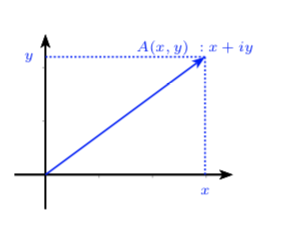
\includegraphics[scale=1]{images/affixe}
\vspace{-0.4cm}
\caption{Plan complexe et affixe}
\end{figure}

\newpage
\paragraph{Somme} : L'addition de deux vecteurs correspond à l'addition des affixes correspondantes: 
%\vspace{1.4cm}
\begin{figure}[h]
\centering
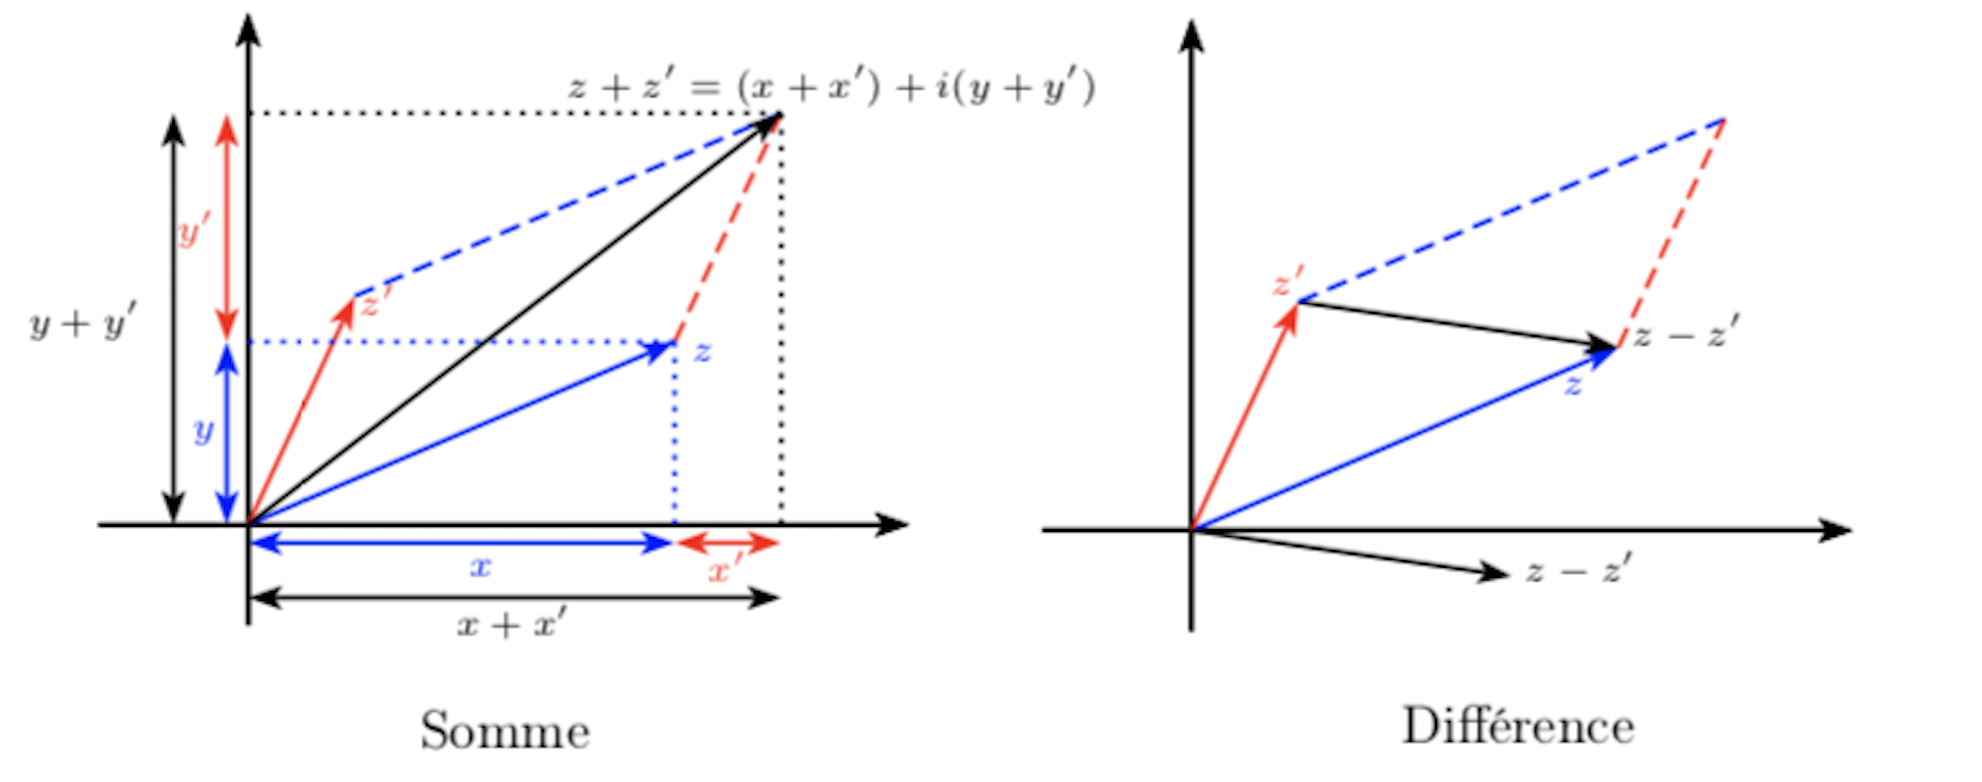
\includegraphics[scale=0.4]{images/somme}
%\vspace{-0.4cm}
%\caption{Somme et différence}
\end{figure}


\paragraph{Multiplication}  par un \underline{réel} $\lambda>0$ correspond à faire une homothétie de rapport $\lambda$. 
\begin{figure}[h]
\centering
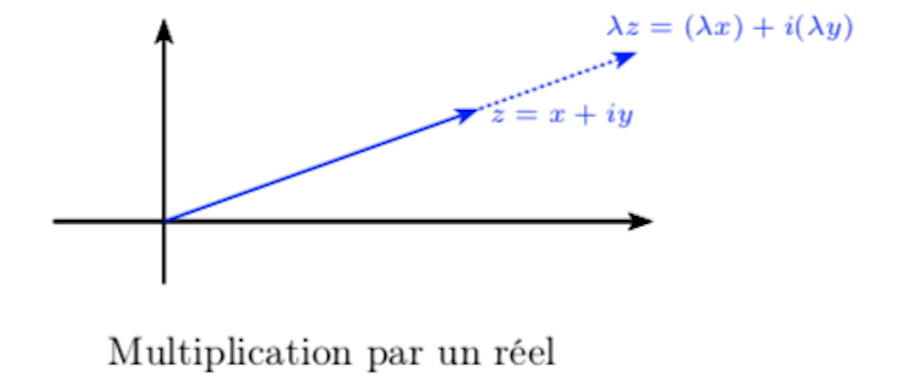
\includegraphics[scale=0.4]{images/mult}
\vspace{-0.4cm}
%\caption{Homothétie}
\end{figure}

\subsection{Conjugué d'un nombre complexe}


\begin{defi}
Soit $z=x+iy$, $(x,y)\in \R^2$ un nombre complexe. On définit le conjugué de $z$ par :
$$\bar{z} =x-iy.$$
\end{defi}
\begin{remarques}
\item $\Re(\bar{z}) =\Re(z)$ et $\Im(\bar{z}) =-\Im(z)$
\item Géométriquement cela correspond à faire une symmétrie par rapport à l'axe des abscisses :

\begin{figure}[h]
\centering
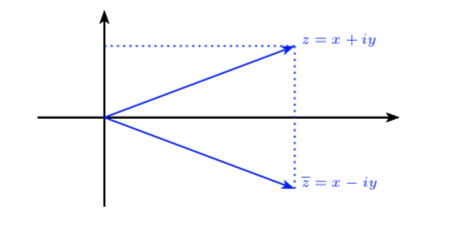
\includegraphics[scale=0.8]{images/conjugue}
\vspace{-0.4cm}
\caption{Conjugué}
\end{figure}
\end{remarques}


\begin{prop}
\begin{enumerate}
\item La conjugaison est \textbf{involutive} : $\forall z\in \bC, \bar{\bar{z}} =z$.
\item La conjugaison est \textbf{linéaire } : 
$$\forall z,z'\in \bC,  \, \forall \lambda\in \R,\,  \bar{z+z'} =\bar{z}+\bar{z'} \quad\text{et} \quad  \bar{\lambda z} =  \lambda \bar{z}.$$
\item La conjugaison  passe au produit et au quotient 
$$\forall z,z'\in \bC,  \,\bar{zz'} =\bar{z}\bar{z'},$$
$$\forall z,z'\in \bC, z'\neq 0 \,\bar{\left(\frac{z}{z'}\right)} =\frac{\bar{z}}{\bar{z'}}.$$
\end{enumerate}
\end{prop}


\begin{prop}
 Pour tout $z \in \bC$ on a 
$$\Re(z) = \frac{1}{2} (z+\bar{z})$$
$$\Im(z) = \frac{1}{2i} (z-\bar{z})$$
\end{prop}
\warning \, Ne pas oubliez la division par $i$ dans la partie imaginaire. 
\begin{figure}[h]
\centering
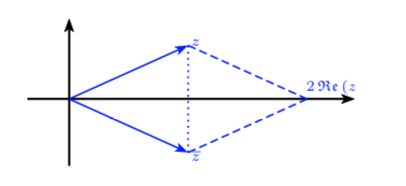
\includegraphics[scale=0.8]{images/reel}
\vspace{-0.4cm}
\caption{Interpretation graphique $\Re(z) = \frac{1}{2} (z+\bar{z})$}
\end{figure}


\begin{figure}[h]
\centering
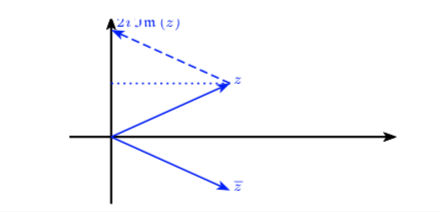
\includegraphics[scale=0.8]{images/imag}
\vspace{-0.4cm}
\caption{Interpretation graphique $\Im(z) = \frac{1}{2i} (z-\bar{z})$ }
\end{figure}

\begin{prop}
$$(z\in \R) \Longleftrightarrow (z=\bar{z})$$ 
$$(z\in i\R) \Longleftrightarrow (z=-\bar{z})$$ 
\end{prop}





\section{Forme trigonométrique}

\subsection{Module d'un nombre complexe}
\begin{defi}
Pour tout nombre complexe $z=x+iy$,  $(x,y)\in \R^2$, on définit le module de $z$ par:
$$|z| = \sqrt{x^2+y^2}.$$
\end{defi}

\begin{remarques}
\item Sur $\R$ le module et valeur absolue coïncident, ce pourquoi on utilise la même notation.
\item $\forall z\in \bC$, $|z| \geq 0$, de plus  $|z| =0$ si et seulement si $z=0$.
\item $\forall z,z'\in \bC^2$, $|z-z'| =0$ si et seulement si $z=z'$.
\item  Le module correspond à la norme du vecteur définie par le point d'affixe $z$. 
$|z-z'|$ désigne la distance entre les points d'affixes $z$ et $z'$. 
\begin{figure}[h]
\centering
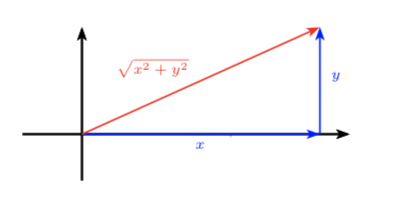
\includegraphics[scale=0.8]{images/module}
\vspace{-0.4cm}
\caption{Interpretation graphique du module }
\end{figure}
\end{remarques}

\begin{prop}
%\begin{enumerate}

$\forall z,z'\in \bC^2$,  $|zz'| =|z| |z'| $ et pour $z'\neq 0$ : 
$\left|\frac{z}{z'}\right| =\frac{|z|}{|z'|}$
%\end{enumerate}

\end{prop}

\begin{prop}
Pour tout $z\in \bC$ :
$$ z \bar{z} =|z|^2 \quad \text{ et } \quad |\bar {z} |= | z|.$$
\end{prop}

IL n'y a pas d'ordre sur $\bC$ (qui généralise l'ordre sur $\R$ et qui est compatible avec les opérations de base).\underline{ Pour obtenir des inégalités on doit être  sur $\R$}
\begin{prop}
Pour tout $z\in \bC$ :
$$ |\Re(z)|\leq |z| \quad \text{ et } \quad |\Im({z}) |\leq  | z|.$$
\end{prop}


\begin{prop}
\begin{enumerate}
\item (Inégalité triangulaire sur $\bC$.) 
$$ \forall z, z' \in \bC^2, \, |z+z'| \leq |z|+|z'|.$$
L'égalité a lieu si et seulement si il existe $\lambda \in \R^+$ tel que $z =\lambda z'$ ou si $z'=0$.
\item Soit $(z,z') \in \bC^2$, on a  :
$$\Big| |z|-|z'|\Big| \leq |z-z'|$$
\end{enumerate}
\end{prop}



\subsection{Cercle trigonométrique}

\begin{defi}
Le \emph{cercle trigonométrique} est le cercle du plan de rayon $1$ et de centre $(0,0)$. 
\end{defi}
\begin{figure}[h]
\centering
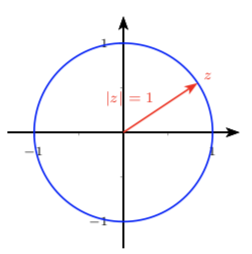
\includegraphics[scale=0.8]{images/cercletrigo}
\vspace{-0.4cm}
\caption{Cercle trigonométrique.}
\end{figure}

\begin{prop}
Dans $\R^2$ le cercle trigonométrique peut se paramétrer de la manière suivante : 
$$\C = \{ (x,y) \in \R^2\, |\, x^2+y^2=1\}.$$
Avec les nombres complexes il peut se paramétrer de la manière suivante : 
$$\C = \{ z \in \bC\, |\, |z|=1\}.$$
\end{prop}



\subsection{Argument d'un nombre complexe}
\begin{defi}
Pour un point du cercle trigonométrique on définit son \emph{argument} par la longueur algébrique de l'arc entre le point $1+0i$  et le point $z$. Le sens positif est choisi de tel sorte que l'argument de $i$ est égal à $\frac{\pi}{2}$ .

Cette unité est le \emph{radian}. 
\end{defi}
\begin{figure}[h]
\centering
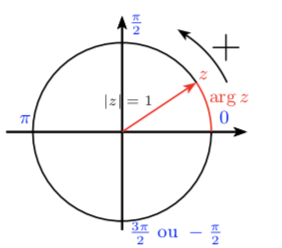
\includegraphics[scale=0.8]{images/orient}
\vspace{-0.4cm}
\caption{Cercle trigonométrique orienté.}
\end{figure}


\begin{defi}
Pour nombre complexe non nul $z\in \bC$, on définit son argument comme l'argument de $\frac{z}{|z|}$. 
\end{defi}
\begin{remarques}
\item L'argument n'est pas défini pour $0$.  
\item L'argument n'est défini qu'à $2\pi$ près. On appelle \emph{argument principal} l'unique argument dans $]-\pi , \pi]$, on le note 
$\arg(z)$
\item Deux nombres complexes sont égaux si et seulement si ils ont le même module et le même argument principal (ou si ils sont nuls tous les deux). 
\end{remarques}

\begin{prop}
Pour tout $z\in \bC^*$ et tout $\lambda \in \R^+$ on a 
\begin{enumerate}
\item $\arg(-z)= \arg(z) +\pi \quad  [2\pi] $
\item $\arg(\bar{z})= -\arg(z) \quad  [2\pi] $
\item $\arg(\lambda z)= \arg(z)  $
\item $\arg(z)= \arg(z') \quad [2\pi]$ si et seulement si $\frac{z}{z'} \in \R^*_+$ 
\item $\arg(z)= \arg(z') \quad [\pi]$ si et seulement si $\frac{z}{z'} \in \R^*$ 
\end{enumerate}

\end{prop}
\begin{exo}
Exprimer $\arg\left( \frac{1}{z}\right) $ en fonction de $\arg(z)$
\end{exo}

Interprétation géométrique : 
Soit $A$ et $B$ deux points du plan d'affixes  respectives $z_A$ et $z_B$. On a 
$$\arg\left( \frac{z_B}{z_A}\right) =\arg(z_B)-\arg(z_A) = \text{l'angle } OA OB$$ 


\subsection{Forme trigonométrique}
\begin{theorem}
Soit $z\in \bC^*$, alors $z$ s'écrit de manière unique sous la forme 
$$z = \rho(\cos(\theta) +i \sin(\theta)), $$
avec $\rho>0$ et $\theta \in ]-\pi, \pi]$. 

Cette écriture est appelée forme trigonométrique de $z$.
\end{theorem}

\begin{proof}
$\frac{z}{|z|}\in U$, on pose
$\theta = \arg(z)=\arg(\frac{z}{|z|})$, on a $\cos(\theta) =\Re(\frac{z}{|z|})$ et $\sin(\theta)= \Im(\frac{z}{|z|})$.
Ainsi $$z = |z| (\cos(\theta) +i \sin(\theta))$$
\end{proof}

\paragraph{Exemple :}  Mettre $z= -3+\sqrt{3}i $ sous forme trigonométrique. 





\section{Forme Exponentielle}
\subsection{Exponentielle complexe}
\begin{defi}
Pour tout $\theta \in \R$  on note 
$$e^{i\theta} =\cos(\theta) +i \sin(\theta).$$
\end{defi}
\begin{remarques}
\item $e^{i\theta}$ est le point du cercle trigonoùétrique d'argument $\theta$. 
\end{remarques}


\begin{figure}[h]
\centering
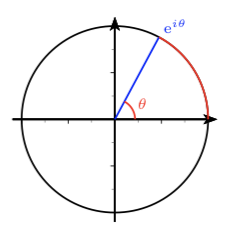
\includegraphics[scale=0.8]{images/eitheta}
\vspace{-0.4cm}
\caption{Représentation de $e^{i\theta}$.}
\end{figure}


\paragraph{Exemples :}
$$e^{i0}=1\quad e^{i\pi} =-1\quad e^{i\pi/2} =i.$$ 

\begin{prop}
\begin{enumerate}
\item $\forall \theta \in \R, \forall k\in \Z, \, e^{i\theta+2k\pi} =e^{i\theta}$
\item $\forall \theta , \theta'\in \R^2,  \, e^{i(\theta+\theta')} =e^{i\theta}e^{i\theta'}$
\item $\forall \theta \in \R,\, \frac{1}{e^{i\theta}} =e^{-i\theta}=\bar{e^{i\theta}}$
\item $\forall \theta \in \R, \forall n\in \Z, \, \left(e^{i\theta}\right)^n =e^{in\theta}$
\item $\forall \theta \in \R, , \, |e^{i\theta}| =1$
\item $U = \{ e^{i\theta} | \theta \in \R\} = \{ e^{i\theta} | \theta \in ]-pi, \pi]\}$
\end{enumerate}
\end{prop}

\begin{proof}
(2)
\end{proof}

\begin{defi}
Soit $\lambda \in \R$ et $\theta \in \R$ on pose : 
$$e^{\lambda +i\theta} =e^{\lambda} e^{i\theta}.$$
\end{defi}
\begin{remarques}
\item On aurait pu dire $\forall z=x+iy \in \bC$, $(x,y)\in \R^2$ on pose
$$e^z =e^{x}e^{iy}.$$
\end{remarques}

\begin{prop}
Pour tout $z, z'\in \bC$ on a 
$$e^{z+z'}=e^{z}e^{z'} \quad \text{ et } \quad \frac{1}{e^z} =e^{-z}.$$
Pour tout $n\in \Z$:
$$\left( e^{z}\right)^n=e^{zn}.$$
\end{prop}

\subsection{Forme exponentielle}
\begin{theorem}
Soit $z\in \bC^*$, $z$ s'écrit de manière unique sous la forme 
$$z = \rho e^{i\theta}$$
avec $\rho>0$ et $\theta \in ]-\pi, \pi]$. 
Cette écriture s'appelle la forme exponentielle de $z$. 
\end{theorem}
\begin{remarques}
\item Soit $z = \rho e^{i\theta}$ sous forme trigonométrique. On a alors 
$$\rho =|z| \quad \text{ et } \theta =\arg(z).$$
\item Multplier par un nombre de la forme $ \rho e^{i\theta}$ revient géométriquement à faire une rotation d'angle $\theta$ et une homothétie de rapport $\rho$. 
\end{remarques}

\begin{prop}
Pour tout $z,z'\in \bC^*$:
$$\arg(zz') =\arg(z)+arg(z') \quad [2\pi]$$
$$\arg(\frac{z}{z'}) =\arg(z)-arg(z') \quad [2\pi]$$
\end{prop}





\section{Application des nombres complexes}


\subsection{Polynôme de degré $2$}
Les nombres complexes permettent de résoudre toutes les équations polynomiales du second degré. 

\begin{theorem}
Soit $P(z)=az^2+bz+c$ un polynome de degré 2 (ie $a\neq 0$) à coefficients réels. $P$ posséde 2 racines (avec multiplicité) dans $\bC$. Plus précisément on a la trichotomie suivante, selon le signe du discriminant  $\Delta =b^2-4ac$ :
\begin{itemize}
\item Si \underline{$\Delta >0$} Alors $P$ admet deux racines réelles distinctes : $$r_1 = \frac{-b +\sqrt{\Delta}}{2a}\quadet r_2 = \frac{-b -\sqrt{\Delta}}{2a} $$
\item Si \underline{$\Delta =0$} Alors $P$ admet une racine réelle (double)  $$r= \frac{-b }{2a}$$

\item Si \underline{$\Delta <0$} Alors $P$ admet deux racines complexes distinctes : $$r_1 = \frac{-b +i\sqrt{-\Delta}}{2a}\quadet r_2 = \frac{-b -i\sqrt{-\Delta}}{2a} $$
\end{itemize}


\end{theorem}

\begin{theorem}
Soit $P(x)=ax^2+bx+c$ un polynôme  de degré $2$. Soit $r_1, r_2$ ses racines (possiblement $r_1=r_2$) . On a alors : 
$$P(x) = a(x-r_1)(x-r_2)$$

En particulier, $r_1r_2= \frac{c}{a}$ et $r_1+r_2=\frac{-b}{a}$

\end{theorem}

Ces résultats se généralisent doublement : 
\begin{itemize}
\item Aux polynômes à coefficients complexes.
\item Aux polynômes  de degré quelconque. 
\end{itemize}

Le théorème suivant est une des bases de l'algébre moderne : 
\begin{theorem}[D'alembert Gauss]
Soit $P$ un polynôme de degré $n$ à coefficients complexes. Alors $P$ admet exactement $n$ racines dans $\bC$ (à multiplicité prés). 

En particulier, tout polynôme non constant admet au moins une racine dans $\bC$.
\end{theorem}


Dans le cours de BCPST, on s'intéressera à une petite généralisation, à savoir la résolution des équations polynomiales du type : 
$$z^2=a$$
avec $a\in \cB$. 

La notion de racine n'est pas bien définie dans $\bC$ car il n'y a pas de relation d'ordre. Dans $\bR$ on a choisi, par convention de prendre la racine positive, mais il n'est pas possible de faire un tel choix dans $\bC$. Ainsi on ne notera jamais racine (z) avec le symbole racine. 

Comment faire alors pour résoudre $z^2=a$ ? L'idée est de mettre $a$ sous forme exponentielle puis de 'deviner' les solutions. 

\begin{theorem}
Soit $a$ un nombre complexe non nul, et $\rho\in \R_+, \theta\in \R$ tel que $a=\rho e^{i\theta}$. L'équation  $z^2=a$ admet alors deux solutions : 
$$z_1 = \sqrt{\rho} e^{\frac{i\theta}{2}} \quadet z_2 = -\sqrt{\rho} e^{\frac{i\theta}{2}}  =\sqrt{\rho} e^{\frac{i\theta +i2\pi}{2}} $$
\end{theorem}

\paragraph{Exemples}
Résoudre dans $\bC$ les équations suivantes :
\begin{itemize}
\item  $z^2=1+i$ 
\item $z^3-z^2+z-1=0$
\item $z^2=\frac{2+2i}{1-i}$
\end{itemize}






\subsection{Trigonométrie}
\begin{prop}
$\forall \theta \in \R$ 
$$\cos(\theta) =\Re(e^{i\theta}) \quad \text{ et } \quad \sin(\theta) =\Im(e^{i\theta}).$$
\end{prop}

\begin{prop}[Formule d'Euler]
$\forall \theta \in \R$ 
$$\cos(\theta) =\frac{e^{i\theta}+e^{-i\theta}}{2} \quad \text{ et } \quad \sin(\theta) =\frac{e^{i\theta}-e^{-i\theta}}{2i} ).$$
\end{prop}
$\warning \, $ Ne pas oublier le $i$ au dénominateur 


\paragraph{Angle moitié}
$\forall (a,b)\in \R^2$, 
$$e^{ia}+e^{ib} = e^{i\frac{a+b}{2}} \left( e^{i\frac{a-b}{2}} +e^{-i\frac{a-b}{2}}  \right) =2\cos\left( {\frac{a-b}{2}} \right) e^{i\frac{a+b}{2}} $$


\begin{exo}
Pour $\theta \notin 2\pi \Z$ simplifier l'expression 
$\frac{1-e^{i\theta}}{1-e^{i\theta}}$
\end{exo}

\begin{prop}[Formule de Moivre]
Soit $\theta\in \R$, et $n\in \Z$:
$$(\cos(\theta)+i\sin(\theta))^n =\cos(n\theta)+i\sin(\theta)$$
\end{prop}

\paragraph{Linéarisation}
La formule de Moivre permet de \emph{linéariser} les formules avec $\sin $ et $\cos$, c'est-à-dire passer de $\cos^p(\theta)\sin^q(\theta)$ à une somme contenant que des termes de la forme $\cos(n\theta)$ et $\sin(n\theta)$. 
\begin{itemize}
\item[$\bullet$] On utilise la formule d'Euler : 
$$\cos^p(\theta)\sin^q(\theta) = \left( \frac{e^{i\theta}+e^{-i\theta}}{2}\right)^p  \left( \frac{e^{i\theta}-e^{-i\theta}}{2i}\right)^a.$$
\item[$\bullet$] On développe avec la formule du binôme de Newton. 
\item[$\bullet$] On rassemble les termes de même exposant pour retrouver des $\sin$ et $\cos$. 
\end{itemize}

\begin{exo}
Pour $\theta \in \R$, linéariser $\sin^5(\theta)$. 
Pour $\theta \in \R$, linéariser $\sin^2(\theta)\cos^3(\theta)$. 
\end{exo}

\paragraph{Délinéarisation}
Si on cherche à faire l'opération inverse, passer d'une formule avec des somme de $sin(n\theta)$ et $\cos(n\theta)$ a des produits. (C'est plus rare de vouloir faire ca) 
%\begin{itemize}
%\item[$\bullet$] On utilise la formule d'Euler : 
%$$\cos^p(\theta)\sin^q(\theta) = \left( \frac{e^{i\theta}+e^{-i\theta}}{2}\right)^p  \left( \frac{e^{i\theta}-e^{-i\theta}}{2i}\right)^a.$$
%\item[$\bullet$] On développe avec la formule du binôme de Newton. 
%\item[$\bullet$] On rassemble les termes de même exposant pour retrouver des $\sin$ et $\cos$. 
%\end{itemize}
%
%\begin{exo}
%Pour $\theta \in \R$, linéariser $\sin^5(\theta)$. 
%Pour $\theta \in \R$, linéariser $\sin^2(\theta)\cos^3(\theta)$. 
%\end{exo}



\subsection{Suite récurrente linéaire d'ordre 2}


\section{Racine $n$-eme de l'unité (Hors Programme)}
Hors programme mais tellement classique. 
\begin{defi}
Soit $n\in \N^*$. On appelle racine $n$-ième de l'unité, tout nombre complexe $z\in \bC$ tel que 
$$z^n=1.$$
\end{defi}

\paragraph{Exemples }
\begin{enumerate}
\item Les racines secondes de $1$ sont  les nombres $z=1$ et $z=-1$.
\item Les racines troisièmes de $1$ sont  les nombres $z=1$ et $z=j$ et $z=j^2$.
\end{enumerate}

\begin{theorem}
Pour tout $n\in \N^*$, il y a exactement $n$ racines $n$-ièmes de l'unité. Elles sont données par 
$$U_n =\{ \xi_k =e^{\frac{2ik\pi}{n}}\, |\, k\in \intent{0,n-1}\}.$$
\end{theorem}

\begin{proof}

\end{proof}

\begin{exo}
Pour tout $n\geq 2$, pour tout $k\in \intent{0,n-1},$ on pose $ \xi_k =e^{\frac{2ik\pi}{n}}$,
$$\sum_{k=0}^{n-1} \xi_k =0 \quad \text{ et } \quad \prod_{k=0}^{n-1} \xi_k =(-1)^{n-1}.$$
\end{exo}




\end{document}